\documentclass[10pt]{article}

\usepackage{fullpage}
\usepackage{color}
\usepackage[table]{xcolor}
\usepackage{hyperref}
\usepackage{graphicx}

%%%%%%%%%%%%%%%%
% Miscellaneous
%%%%%%%%%%%%%%%%

\definecolor{primary}{rgb}{0,0,.50}
%\definecolor{primary}{rgb}{0,0,0}
\definecolor{secondary}{rgb}{.7,.5,0}
\definecolor{table-primary}{rgb}{1,1,1}
\definecolor{table-secondary}{rgb}{.975,.99,1}

%%%%%%%%%%%%%%%%
% Title Section
%%%%%%%%%%%%%%%%

\title{\color{primary}\texttt{UCSC Plaza \\ Sprint 2:}}
\author{{\color{secondary}\textbf{Team Amlesh the Great}} \\ Kyungmin So (PO), Youngsoo Jang, \\ Hobin Ryu, Seungwoo Lee \\ Amlesh Sivanantham, and James Garbagnati }
\date{Release: American Bobtail (July 11, 2016) \\ Revision 1.0 (July 11, 2016)}

%%%%%%%%%%%%%%%%%%%%%%
% User-Defined Macros
%%%%%%%%%%%%%%%%%%%%%%

%\ignore = Multiline comments
\newcommand{\ignore}[1]{}

\newcommand{\gobblepagenum}{\thispagestyle{empty}\addtocounter{page}{-1}}

%\fancysec{Section title}{Label} = Fancy, colored and labelled section
% Basically just to make it easier to change the format of the whole doc
% Commands with an X are non-numbered sections
\newcommand{\fancysec}[2] {{\color{primary}\section{#1} \label{sec:#2}}}
\newcommand{\fancysub}[2] {{\color{primary}\subsection{#1} \label{sec:#2}}}
\newcommand{\fancysubsub}[2] {{\color{primary}\subsubsection{#1} \label{sec:#2}}}

\newcommand{\fancysecX}[2] {{\color{primary}\section*{#1} \label{sec:#2}}}
\newcommand{\fancysubX}[2] {{\color{primary}\subsection*{#1} \label{sec:#2}}}
\newcommand{\fancysubsubX}[2] {{\color{primary}\subsubsection*{#1} \label{sec:#2}}}


% P.S. I'm so fancy, you already know


%%%%%%%%%%%%%%%%%
% Begin Document
%%%%%%%%%%%%%%%%%
\begin{document}

\maketitle

\fancysecX{High Level Goals}{goals}

    \begin{itemize}
        \item Create Search and Apply functionality for events.
        \item Allow users to manage Event Settings.
%        \item Search functionality to find events happening within campus.
%        \item Give users the ability to rate and comment to leave feedback on events.
%        \item Suggest similar events to users based on their personal preferences.
    \end{itemize}
    
\fancysecX{User Stories for Release}{stories}
    
    \fancysubX{Sprint 1}{sprint1}
     
        \begin{itemize}
            \item (3) User Story 1: As an event planner, I want to add or delete my events, so that other members of UCSC can see if my event is available.

                \begin{itemize}
                    \item Task 1. Implement Layout. (2 hour)
                    \item Task 2. Send input as json data file. (2 hour)
                    \item Task 3. Insert Event and its details into the database. (2 hour)
                \end{itemize}        
                Total for User Story: 6 hours
            \item (2) User Story 2: As an event-goer, I want to be able to see details of an event, so that I can decide whether or not to go.
            
                \begin{itemize}
                    \item Task 1. Implement layout. (2 hour)
		    \item Task 2. Be able to pull details from the database. (2 hour)
                \end{itemize}
                Total for User Story: 4 hours
            \item (3) User Story 3: As an event-goer, I want to be able to search for specific events, so that I may find the event that I need.
            
                \begin{itemize}
                    \item Task 1. Implement layout. (2 hour)
                    \item Task 2. Send the search query to the server. (3 hour)
		    \item Task 3. Backend should search through the database and produce a list. (3 hour)
                \end{itemize}
                Total for User Story: 8 hours
            \item (1) User Story 4: As an event-goer, I want to be able to see a marker on the map, so that I can see where it is.
            
                \begin{itemize}
                    \item Task 1. Pull location details from the database, and mark it on the map. (2 hour)
                \end{itemize}r
                Total for User Story: 2 hours
            \item (2) User Story 5: As an event-goer, I want to be able to send or rescind an application to a specific event, so that the event planner knows whether I will attend or not.
        
                \begin{itemize}
                    \item Task 1. Make the submit button funcitonal. (1 hour)
		    \item Task 2. Send user info to the event database. (2 hour)
		    \item Task 3. Send confirmation to the user, and show them their current status on the event details page. (2 hour)
		    \item Task 4. Be able to cancel status. (1 hour)
                \end{itemize}
                Total for User Story: 6 hours
	    \item (2) User Story 6: As an event planner, I want to be able to see who applied to my event and be able to accept or decline their application, so that event-goers know if they are allowed to participate or not.

		\begin{itemize}
		    \item Task 1. Recieve the list of users who applied to the event from the server. (1 hour)
		    \item Task 2. Display the list on the event details page with accept and reject options. (2 hour)
		    \item Task 3. Send acceptance status to the server. (1 hour)
		    \item Task 4. Notify applicant of their status. (1 hour)
		\end{itemize}
		Total for User Story: 5 hours
	    \item (1) User Story 7: As an event planner, I want to be able to manage my event, so that I can apply certain constraints to the event.

		\begin{itemize}
		    \item Task 1. Design layout for the management page. (3 hour)
		\end{itemize}
		Total for User Story: 3 hours
        \end{itemize}
     
%    \fancysubX{Sprint 2}{sprint2}
        
%        \begin{itemize}
%            \item (5) User Story 1: As an event planner, I want to be able to manage my event, so that I can apply certain constraints to the event.
%            \item (3) User Story 2: As an event-goer, I want to be able to send or rescind an application to a specific event, so that the event planner knows whether I plan to attend or not.
%            \item (3) User Story 3: As an event planner, I want to see who applied to my event and be able to accept or decline their application, so that the event goers know if they are allowed to partake or not.
%            \item (5) User Story 4: As an event-goer, I may wish for privacy settings, so that I can ensure that my event-attendance is not seen by the public.
%            \item (8) User Story 5: As an event-goer, I want to be able to search for specific events, so that I may apply to attend the event.
%        \end{itemize}
         
%    \fancysubX{Sprint 3}{sprint3}
     
%        \begin{itemize}
%            \item (5) User Story 1: As an event-goer, I want to see the current and maximum attendance for the event, so that I can ensure there is space for me to attend and that it is not overcrowded. 
%            \item (5) User Story 2: As an event-planner, I want to ensure that my event does not exceed maximum attendance, so that my event is not overcrowded and has enough room for all event-goers.
%            \item (3) User Story 3: As an event-goer, I want to be able to see and submit my own rating for an event, so that I can decide to go to an ongoing event or offer my opinion towards the event.
%            \item (3) User Story 4: As an event planner, I want to get some feedback on my event, so that I can improve the experience of my event.
%            \item (8) User Story 5: As an event-goer, I want to be able to socialize over an event, so that I can share my opinion with friends and other participants.
%            \item (21) User Story 6: As an event-goer, I want to be able to see if my friends are going to a certain event, so that I know which events have my friends in it.
%            \item (13) User Story 7: As an event-goer, I want to receive recommendations on other events tailored to my preference, so that I can see events that I may attend in the future.
%        \end{itemize}

\fancysecX{Team Roles}{roles}

    \begin{itemize}
        \item Kyungmin So: Product Owner, Back-end Developer
        \item Youngsoo Jang: Front-end Developer
        \item Hobin Ryu: Scrum Master, Front-end Developer
        \item Seungwoo Lee: Designer
        \item Amlesh Sivanantham: Scrum Master, Front-end Developer
        \item James Garbagnati: Front-end Developer
    \end{itemize}

    \fancysubX{Intial Task Asignment}{intialtask}
        \begin{itemize}
            \item Kyungmin So: User Story 1, Task 3
            \item Youngsoo Jang: User Story 7, Task 1
            \item Hobin Ryu: User Story 3, Task 1
            \item Seungwoo Lee: Designer
            \item Amlesh Sivanantham: User Story 2, Task 1 
            \item James Garbagnati: User Story 1, Task 1
        \end{itemize}

\fancysecX{Initial Burnup Chart}{burnupchart}

    \begin{figure}[!ht]
  	\caption{Burnup Chart at the end of sprint 1}
  	\centering
    		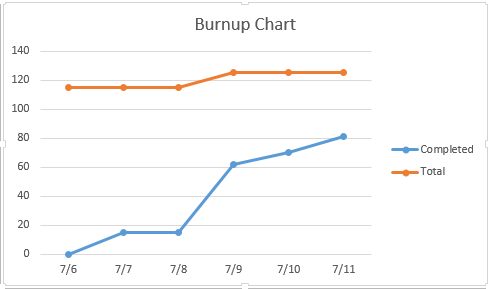
\includegraphics[width=1\textwidth]{Burnupchart1}
    \end{figure}

\vspace{5cm}
\fancysecX{Initial Scrum Board}{scrumboard}

   \begin{figure}[!ht]
  	\caption{Scrum board at the end of Sprint 1}
  	\centering
    		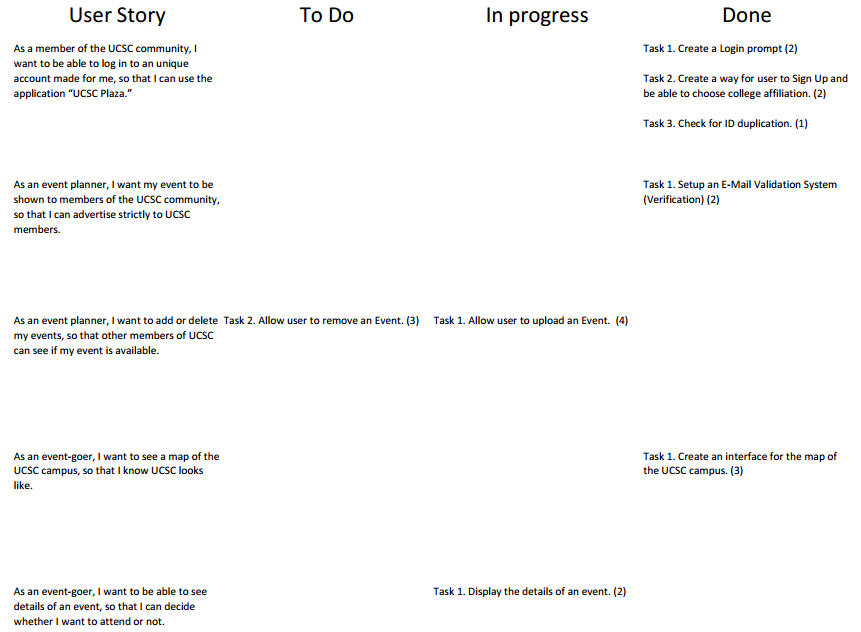
\includegraphics[width=1\textwidth]{scrumboard1}
\end{figure}

\fancysecX{Scrum Times}{scrumTimes}

    We will be meeting on Monday and Wednesday at 4:30 PM, and on Friday and Sunday at 5:00 PM.

\end{document}
